\documentclass[conference]{IEEEtran}
\pdfoutput=1

\usepackage{graphicx}
\usepackage{hyperref}
\usepackage[english]{babel}
\usepackage[utf8]{inputenc}
\usepackage{listings}
\usepackage[table]{xcolor}
\usepackage{pdfpages}

\hypersetup{colorlinks=true,citecolor=[rgb]{0,0.4,0}}


\title{YouTube comment sentiment analysis \\with web interface}
\author{Søren Howe Gersager \\ \IEEEauthorblockN{s094557}
\IEEEauthorblockA{Technical University of Denmark}
\and
Anders Lønberg Rahbek \\ \IEEEauthorblockN{s107029}
\IEEEauthorblockA{Technical University of Denmark}
}

%\author{Søren Howe Gersager - s094557, Anders Rahbek - s107029}
\begin{document}
\maketitle

\begin{abstract}
We have created a webservice that performs sentiment analysis on 
YouTube videos using the Google Data APIs, 
by using a self combined corpus and a trained simple machine learning classifier
\end{abstract}

\section{Introduction}
This paper showcases the results of a project, analyzing YouTube comments using Python. \\
It describes the methods and techniques used to create the analysis and discusses the paths taken as well as further potential work to be done.

\section{Methods}

We have divided the project into classes specific for the different areas our project encompasses: a youtube scraper, a sentiment analyser and a webservice.

\subsection{Webservice}
For the webservice we use the Flask \cite{flask} using the Jinja2 \cite{jinja2} templating engine, this allows us to separate the code from the markup.

We also used Javascript and SASS \cite{sass},  to a lesser degree for the frontend development of the webservice.

While developing we have used the built-in flask web server for ease of use, for deployment however, a traditional web server like Apache with mod\_fastcgi would probably be the better option for its performance and security.

\subsection{Sentiment analyser}
The sentiment analyser is based on the NLTK package \cite{nltk}. We train a Naive Bayes classifier and saves the classifier as a pickle file, so we next time don't  have to train, but simply load the classifier into NLTK. \\
The classifier is trained based on a combined corpus of tweets from Twitter \cite{twitter} and movie reviews \cite{movie_corpus}. \\

The corpus has been pre-prossesed so there is equal number of positive and negative texts - 13333 each. The hashtags and user-specified tags ('@'-tag) has also been removed from the twitter corpus. Reversed, there has been added a few emoticons like ':D' and ':(' (positive and negative respectively).\\

The sentiment analysis itself, is done by a method which takes the comments as input and do sentiment analysis on all of them. Then it's finding a overall classification of the video by making a majority vote of the comments sentiment. The classification can be one of five possibillities: Strong negative, slight negative, neutral, slight positive or strong positive.


\subsection{YouTube scraper}
The YouTube scraper uses the Google Data API's for fetching data from youtube and requests as the library making the HTTP requests. We realize a python gdata module already exists, 

\subsection{General}
The project runs Python 3 and have not been tested on Python 2,
however all external libraries we use has a Python 2 equivalent. 
The only real hurdle for compatibility would be the difference in the Python Standard Library.

In the beginning of the project we simply used the sqlite \cite{sqllite} module for communication with the database, however we later realized this was cumbersome because we had to manually write functions for inserting all the scraped information into the database, we decided to switch to the sqlalchemy object relational mapper \cite{sqlalchemy} for database communication. By using an ORM we saved time and could do database transactions in an easy way using our specified models.

Behind the sqlalchemy ORM we use the sqlite database, as it allows for fast prototyping, Figure ~\ref{fig:database} shows an ER diagram for the database schema.

Code listings can be found in the listings section.

\section{Results}

Figure~\ref{fig:videopage} shows a screenshot of the webservice
with a sentiment analysis analysis of a \href{https://www.youtube.com/watch?v=YESZ1S1zLW}{YouTube video}.\\

\subsection{Sentiment analysis}
Our sentiment analysis showed an accuracy of 68.58\%, which is decent. This result is based on a test-set and by using util.accuracy in the NLTK package. \\
The training of the classifier is taking some time. This time is way too long if it should train every time (approx. 40 minutes). This is touched upon further in the Discussion section. 
 
\begin{figure}[a]
\centering
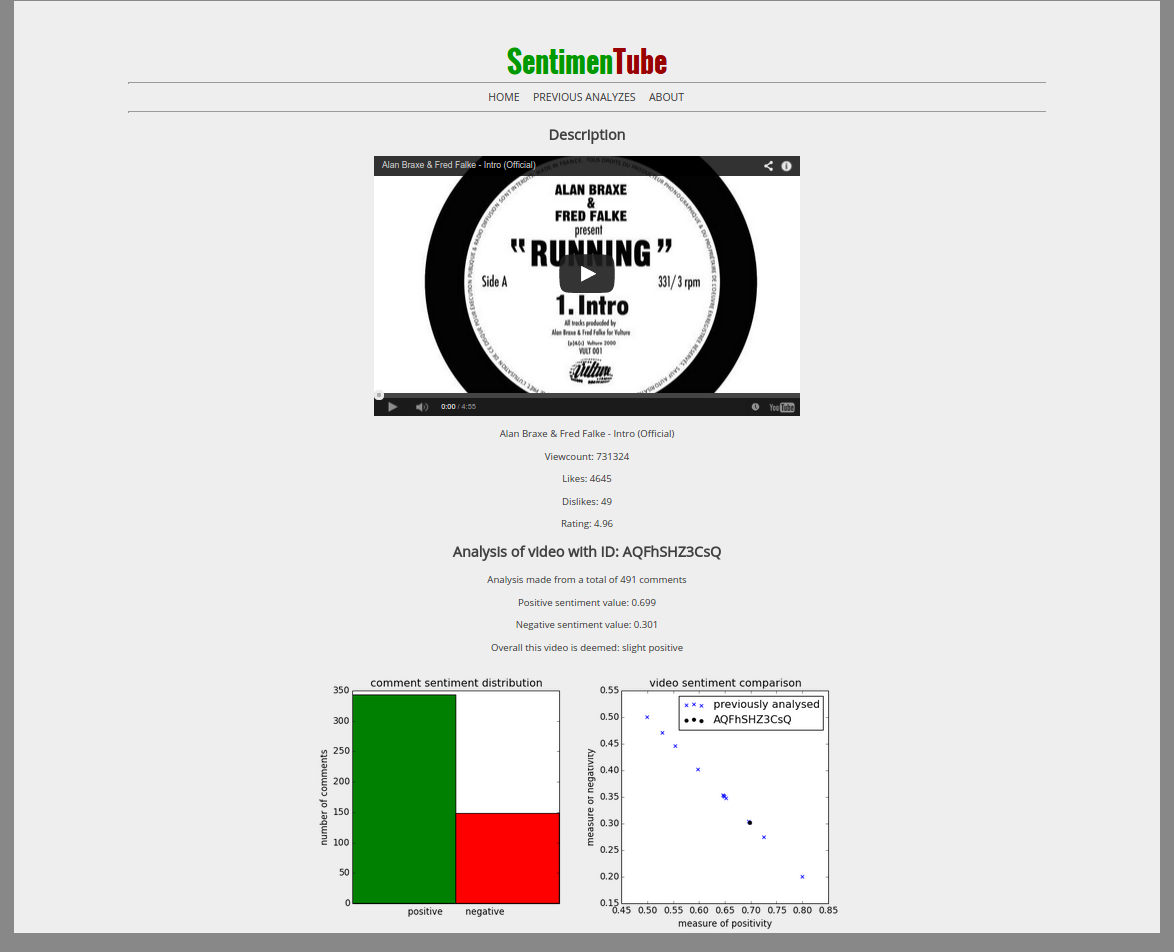
\includegraphics[width=\columnwidth]{video.png}
\caption{Result of sentiment analysis of YouTube video}
\label{fig:videopage}
\end{figure}

\begin{figure}[b]
\centering
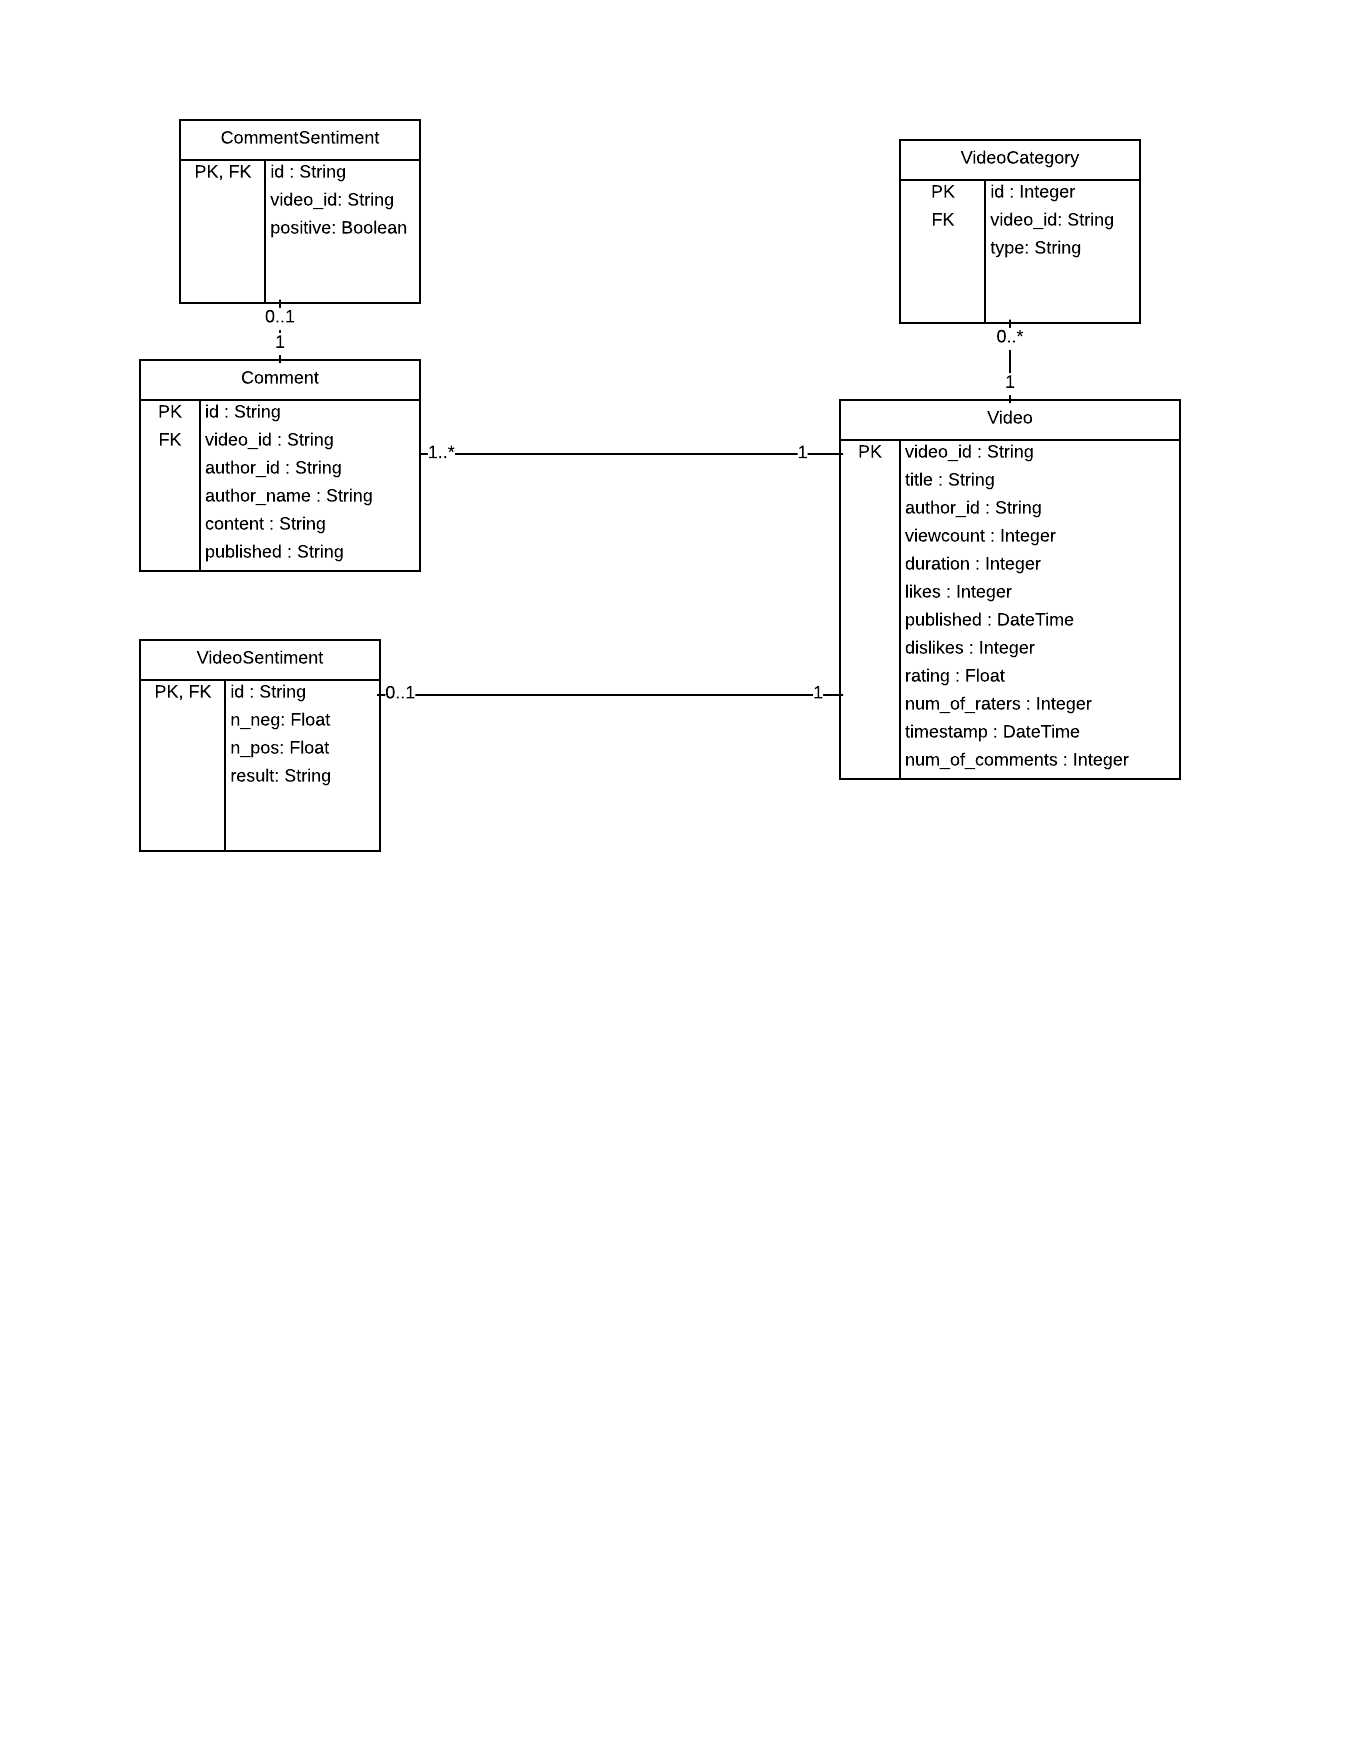
\includegraphics[width=\columnwidth]{database.png}
\caption{Database schema}
\label{fig:database}
\end{figure}


\subsection{Code checking}
For syntax and static checking we used flake8\cite{flake8}, a wrapper of pyflakes and pep8, we also used pylint\cite{pylint} and pep257\cite{pep257}.
We integrated these checks as a part of our testing so we could quickly assess if our code was sound.  
In addition to checking our code we also checked our tests.

\subsection{Testing}
For testing we primarily used the python unittest library in combination with nose \cite{nose}, we used coverage \cite{coverage} for code coverage making sure we had a test coverage of 100\%. 
As written above we integrated the flake8 and pylint checking into the tests.
We used both unit-testing and integration testing in testing the various components in our project.
We have divided the tests into several files where each test file corresponds to a module and one for the code checking tests.


\subsection{Profiling}

We have not analysed the project by profiling but we estimate the HTTP requests and the classification performed will be the bottleneck. This is touched upon further in the Discussion section.

\section{Discussion}

As our sentiment corpus consists of words in english, the sentiment analysis will only work for English texts.

As the webservice makes use of the Google Data APIs it has to make several HTTP GET requests for fetching comments, right now 1 request for every 25 comments, this serves as a bottleneck for analysing YouTube videos with large amounts of comments. Because of this bottleneck it results in a delay for the user the first time a new video is analysed, however subsequent requests on the particular video will fetch the information from the database eliminating the delay. The database fetch happens only if the number of comments for the video are unchanged from the last analysis. Further work could be spent looking into optimizing the HTTP requests made for example by parallelization of the requests. The classification also take up a considerable amount of time and further time could be spent optimizing this as well. Profiling the project could be done using the cProfile module\cite{cprofile}.\\

As mentioned earlier, the training of the classifier is taking too long. As we saves the classifier, so we next time just can load it, it's something we can live with.  \\ 
By reducing the corpus, we can cut down the training time. But this will affect the accuracy of the classifier. So it's a trade-off issue. As we don't know exactly how much the trade-off is and how much of the corpus we can cut-off before the accuracy of the classifier is decreasing too much, this is an area to look into the next step to go for optimizing the sentiment analysis. 

\section{Conclusion}
We have implemented a YouTube sentiment web service mining YouTube comments and performing sentiment analysis. \\
By using a simple Naive Bayes classifier and relative big corpus, we obtained a decent accuracy of 68.58\%\\
Due to the nature of the service and restrictions in the Google Data APIs it works best with a small number of comments, however we mediate it somewhat by saving the results to a local database.

\bibliographystyle{IEEEtran}
\bibliography{references.bib}


\clearpage
\onecolumn
\appendices
\section{Code listings}

\definecolor{darkgreen}{rgb}{0, 0.4, 0}
\lstset{language=Python,
  numbers=left,
  frame=bottomline,
  basicstyle=\scriptsize,
  identifierstyle=\color{blue},
  keywordstyle=\bfseries,
  commentstyle=\color{darkgreen},
  stringstyle=\color{red},
  inputencoding=utf8
}
\lstset{literate=%
{ï}{{\"i}}1
{ø}{{\"o}}1}
\lstlistoflistings

\label{listing:youtube}\lstinputlisting{../sentimentube/youtube.py}
\label{listing:sentiment_analysis}\lstinputlisting{../sentimentube/sentiment_analysis.py}
\label{listing:webserve}\lstinputlisting{../sentimentube/webserve.py}
\label{listing:models}\lstinputlisting{../sentimentube/models.py}
\label{listing:database}\lstinputlisting{../sentimentube/database.py}

\label{listing:test_flask}\lstinputlisting{../test/test_flask.py}
\label{listing:test_youtube}\lstinputlisting{../test/test_youtube.py}
\label{listing:test_sentiment_analysis}\lstinputlisting{../test/test_sentiment_analysis.py}
\label{listing:test_codeformat}\lstinputlisting{../test/test_codeformat.py}

\newpage
\section{Automatic generation of documentation}

Demontration using epydoc:
\begin{verbatim}
epydoc --pdf -o /home/fnielsen/tmp/epydoc/ --name RBBase wikipedia/api.py
\end{verbatim}
Test output (nosetests): 
\begin{verbatim}
nose.config: INFO: Ignoring files matching ['^\\.', '^_', '^setup\\.py$']
nose.plugins.cover: INFO: Coverage report will include only packages: ['youtube', 'webserve', 'sentiment_analysis', 'database']
nose.selector: INFO: /home/syre/Dropbox/opgaver/Kandidat/02819 Data mining med Python/datamining-with-python/epydoc_script.sh is executable; skipped
Test the modules for flake8 violations. ... ok
Test the modules for pep257 violations. ... ok
Test the modules for pylint violations. ... ok
Test about page loads correctly. ... ok
Test that webservice fails gracefully on wrong url. ... ok
Test that the previous page shows the 5 most recent analyses. ... ok
Test that the start page is loading correctly. ... ok
Test asserting the comment sentiment plot works (mixed). ... ok
Test asserting the comment sentiment plot works (with negative). ... ok
Test asserting the comment sentiment plot works (with positive). ... ok
Test edge-case: video with comments disallowed. ... ok
Test edge-case: video with no comments. ... ok
Test that video loads from database directly if found. ... ok
Test that fetches youtube information and loads video page. ... ok
Test of video page with URL. ... ok
Test that tries to input an invalid video id at the start page. ... ok
Test asserting comments are saved after video page load. ... ok
Test asserting comment sentiments are saved after video page load. ... ok
Test asserting video is saved in database after video page load. ... ok
Test asserting a videosentiment is saved after video page load. ... ok
Test for "outdated" video in database. ... ok
Test that video sentiment on video page load works correctly. ... ok
Test the classify_comment method in sentiment_analysis. ... ok
Test the eval method in sentiment_analysis. ... ok
Test the load_classifier method. ... ok
Test load method. ... ok
test _comment_generator handles wrong video_id. ... ok
test of fetch_comments in YouTubeScraper with correct id. ... ok
test fetch_comments returning all comments unexplicitly. ... ok
test of fetch_comments returning all comments correctly. ... ok
test fetch_videoinfo handles wrong video_id. ... ok
test in case of requests error. ... ok

Name                 Stmts   Miss  Cover   Missing
--------------------------------------------------
database                11      0   100%   
sentiment_analysis     104      0   100%   
webserve               116      0   100%   
youtube                 86      0   100%   
--------------------------------------------------
TOTAL                  317      0   100%   
----------------------------------------------------------------------
Ran 32 tests in 93.541s

OK

\end{verbatim}
%\includepdf[pages={-}]{/home/fnielsen/tmp/epydoc/api.pdf}

\end{document}
